\chapter{Two-Person bargaining}

\section{Nash Bargaining Solution}

Let $X$ be the set of possible outcomes. Let $U$ be the set of feasible expected utilities from $X$, which is assumed to be a compact and convex subset of $\RR^2$. Let $d\in U$ be the disagreement point, which is the outcome if the two parties fail to reach an agreement. We assume that $\exists u\in U$ such that $u \gg d$ (i.e., there is some outcome that is strictly better than the disagreement point for both parties).
A bargaining solution is a function $F$ that maps $(U, d)$ to a point $F(U,d)\in U$.

\state{Requirement: Scale Invariance}{
  Consider the transformation $(U,d)\mapsto (\bar U,\bar d)$ such that
  \[
  \begin{aligned}
    \bar U & = \brace{(\bar u_1,\bar u_2)\bigg| \bar u_i = \alpha_i u_i+\beta_i \text{ for some }\alpha_i>0,\quad (u_1,u_2)\in U},\\
    \bar d_i & = \alpha_i d_i + \beta_i.
  \end{aligned}
  \]
  Then,
  \[
  F_i(\bar U,\bar d) = \alpha_i F_i(U,d) + \beta_i.
  \]
}

\state{Requirement: Efficiency}{
  $\nexists u\in U$ such that $u \gg F(U,d)$.
}

\state{Requirement: Symmetry}{
  If $U$ is symmetric (i.e., $(u_1,u_2)\in U\iff (u_2,u_1)\in U$) and $d_1 = d_2$, then 
  \[
  F_1(U,d) = F_2(U,d).
  \]
}

\state{Requirement: Independence of Irrelevant Alternatives (IIA)}{
  Consider $(U,d)$ and $(\bar U,d)$ such that $U\subseteq \bar U$. If $F(\bar U,d) \in U$, then,
  \[
  F(\bar U,d) = F(U,d).
  \]
}

\thmp{}{
  There is one and only one $F$ that satisfies the above requirements. $F$ is given by:
  \[
  F^N(U,d) = \argmax_{u\in U, u\ge d} (u_1 - d_1)(u_2 - d_2).
  \]
}{
  Firstly, it is easy to check that $F^N$ is well-defined in the sense that $F^N$ satisfies the above requirements.

  Let $(u_1^*, u_2^*) = F^N(U,d)$. We can always rescale the utilities such that $(u_1^*,u_2^*) \mapsto (1,1)$ and $(d_1,d_2) \mapsto (0,0)$, without loss of generality. Denote the new space as $(\bar U,\bar d)$.

\begin{center}
  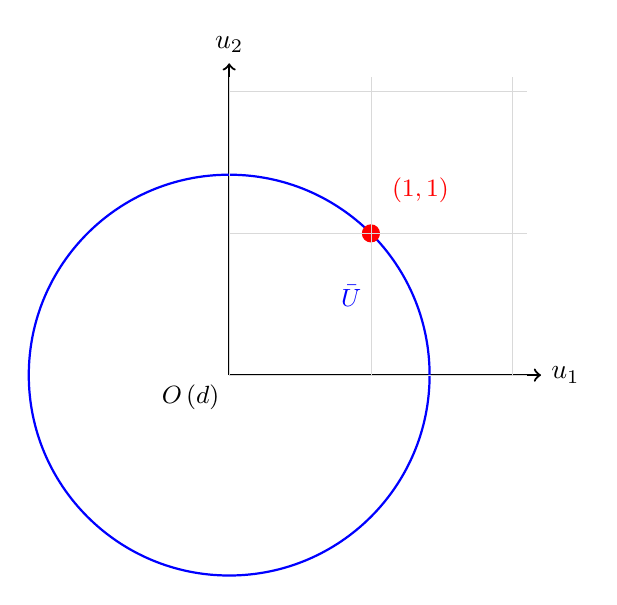
\begin{tikzpicture}[scale=1.8]
    % Axes
    \draw[->,thick] (0,0) -- (2.2,0) node[right] {$u_1$};
    \draw[->,thick] (0,0) -- (0,2.2) node[above] {$u_2$};
    
    % Origin label
    \node[below left, font=\small] at (0,0) {$O\, (d)$};
    
    % Circle centered at origin with radius sqrt(2) ≈ 1.414
    \draw[thick, blue] (0,0) circle [radius=1.414];
    \node[blue, below left, font=\small] at (1.0, 0.7) {$\bar U$};
    
    % Point (1,1) on the circle
    \draw[red, fill=red] (1,1) circle [radius=0.06];
    \node[red, above right, font=\small] at (1.08, 1.15) {$(1,1)$};
    
    
    % Add grid for reference
    \draw[very thin, gray!30] (0,0) grid (2.1, 2.1);
    
\end{tikzpicture}
\end{center}
\clmp{}{
  If we can show that $F = F^N$ for any $F$ in the scaled space $(\bar U, \bar d)$, then we must have $F = F^N$ for any $(U,d)$.
}{
  This is true by scale invariance.
}

  \clmp{}{
    $F^N(\bar U,d) = (1,1)$.
  }{
    Define the set $H = \brace{(u_1,u_2)\,|\,u_1+u_2\le 2}$.
    Note that the boundary of $H$ is the tangent line to the hyperbola $u_1 u_2 = 1$ through $(1,1)$ with slope -1. Since $(1,1)\in \bar U$ and $(1,1)\in H$, if we can show that $\bar U\subseteq H$, then we must have $(1,1)$ as the solution.
\begin{center}
  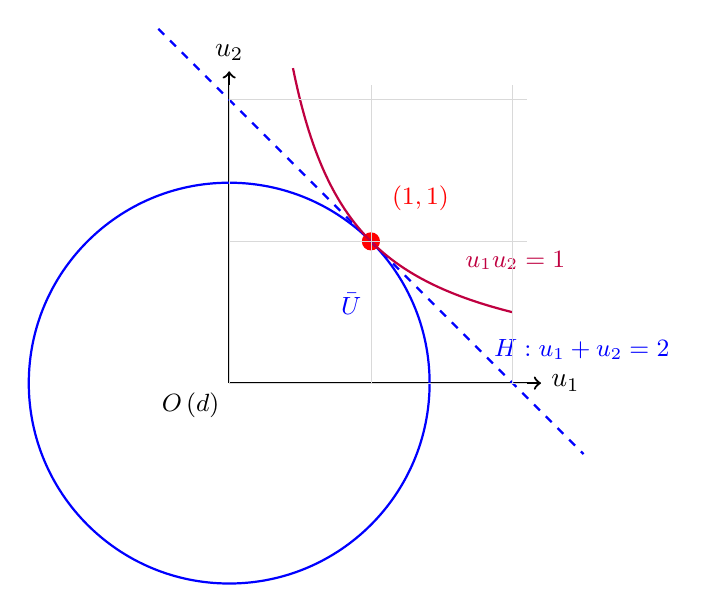
\begin{tikzpicture}[scale=1.8]
    % Axes
    \draw[->,thick] (0,0) -- (2.2,0) node[right] {$u_1$};
    \draw[->,thick] (0,0) -- (0,2.2) node[above] {$u_2$};
    
    % Origin label
    \node[below left, font=\small] at (0,0) {$O\, (d)$};
    
    % Circle centered at origin with radius sqrt(2) ≈ 1.414
    \draw[thick, blue] (0,0) circle [radius=1.414];
    \node[blue, below left, font=\small] at (1.0, 0.7) {$\bar U$};
    
    % Point (1,1) on the circle
    \draw[red, fill=red] (1,1) circle [radius=0.06];
    \node[red, above right, font=\small] at (1.08, 1.15) {$(1,1)$};
    
    % Tangent line through (1,1) with slope -1 (dashed)
    \draw[dashed, blue, thick] (-0.5,2.5) -- (2.5,-0.5);
    \node[blue, above right, font=\small] at (1.8, 0.1) {$H: u_1 + u_2 = 2$};
    
    % Hyperbola u_1 u_2 = 1
    % Parametric form: (t, 1/t) for t in suitable range
    \draw[thick, purple] plot[domain=0.45:2.0, samples=100] (\x, {1/\x});
    \node[purple, below right, font=\small] at (1.6, 1) {$u_1 u_2 = 1$};
    
    % Add grid for reference
    \draw[very thin, gray!30] (0,0) grid (2.1, 2.1);
    
\end{tikzpicture}
\end{center}
    To show that $\bar U\subseteq H$, suppose for contradiction that $\bar U$ contains some point $(u_1,u_2)$ such that $u_1 + u_2 > 2$. The line segment connecting $(1,1)$ and $(u_1,u_2)$ must intersect the hypobola $u_1 u_2 = 1$ at some point $(\tilde u_1, \tilde u_2)$. So the line segment joining $(\tilde u_1,\tilde u_2)$ and $(1,1)$ must be above the hypobola $u_1 u_2 = 1$. Since $\bar U$ is convex, we can find a convex combination of $(u_1,u_2)$ and $(1,1)$ that falls within the line segment joining $(\tilde u_1,\tilde u_2)$ and $(1,1)$, denoted by $(\hat u_1,\hat u_2)$ such that $(\hat u_1,\hat u_2)\in \bar U$ and $\hat u_1\hat u_2 > 1$. This contradicts the assumption that $F^N(\bar U,d) = (1,1)$.


\begin{center}
  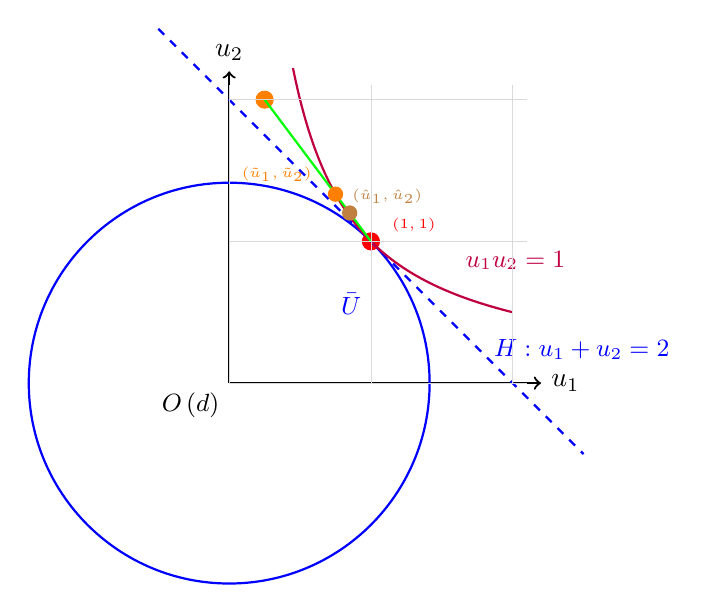
\begin{tikzpicture}[scale=1.8]
    % Axes
    \draw[->,thick] (0,0) -- (2.2,0) node[right] {$u_1$};
    \draw[->,thick] (0,0) -- (0,2.2) node[above] {$u_2$};
    
    % Origin label
    \node[below left, font=\small] at (0,0) {$O\, (d)$};
    
    % Circle centered at origin with radius sqrt(2) ≈ 1.414
    \draw[thick, blue] (0,0) circle [radius=1.414];
    \node[blue, below left, font=\small] at (1.0, 0.7) {$\bar U$};
    
    % Point (1,1) on the circle
    \draw[red, fill=red] (1,1) circle [radius=0.06];
    \node[red, above right, font=\tiny] at (1.08, 1) {$(1,1)$};
    
    % Tangent line through (1,1) with slope -1 (dashed)
    \draw[dashed, blue, thick] (-0.5,2.5) -- (2.5,-0.5);
    \node[blue, above right, font=\small] at (1.8, 0.1) {$H: u_1 + u_2 = 2$};
    
    % Hyperbola u_1 u_2 = 1
    % Parametric form: (t, 1/t) for t in suitable range
    \draw[thick, purple] plot[domain=0.45:2.0, samples=100] (\x, {1/\x});
    \node[purple, below right, font=\small] at (1.6, 1) {$u_1 u_2 = 1$};
    
    % Point outside H on the right: (0.25, 2)
    \draw[orange, fill=orange] (0.25, 2) circle [radius=0.06];
    
    % Line segment connecting (0.25, 2) and (1, 1)
    \draw[green, thick] (0.25, 2) -- (1, 1);
    
    % Intersection point with hyperbola: (0.75, 1.333)
    \draw[orange, fill=orange] (0.75, 1.333) circle [radius=0.05];
    \node[orange, above left, font=\tiny] at (0.65, 1.35) {$(\tilde u_1,\tilde u_2)$};
    
    % Intermediate point on the line segment (closer to (1,1)): (0.85, 1.2)
    \draw[brown, fill=brown] (0.85, 1.2) circle [radius=0.05];
    \node[brown, above right, font=\tiny] at (0.8, 1.2) {$(\hat u_1,\hat u_2)$};
    
    % Add grid for reference
    \draw[very thin, gray!30] (0,0) grid (2.1, 2.1);
    
  \end{tikzpicture}
\end{center}
  }
  
  \clmp{}{
    For any $F$, the solution must be $(1,1)$.
  }{
    We can always include the $\bar U$ using a symmetric right triangle whose hypotenuse is on the boundary of $H$ and whose right angle sits on the line of $u_1 = u_2$. Denote the new triangle by $\bar{\bar U}$.
    
    \vspace{0.4cm}
    
    \begin{center}
      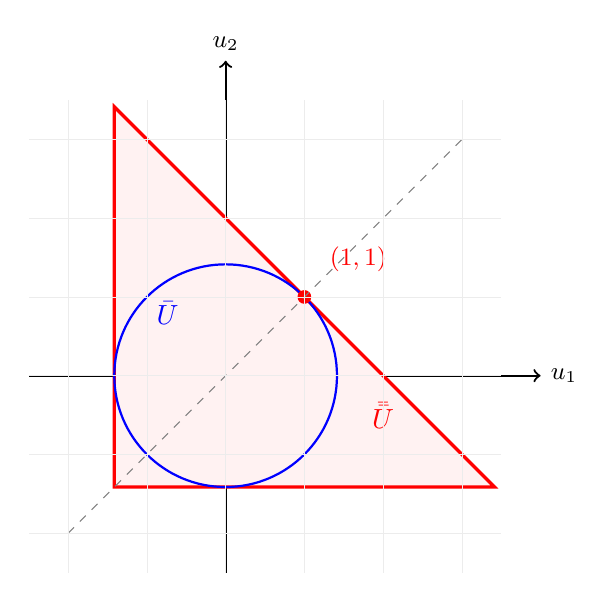
\begin{tikzpicture}[scale=1.0]
        % Axes extended
        \draw[->,thick] (-2.5,0) -- (4,0) node[right, font=\small] {$u_1$};
        \draw[->,thick] (0,-2.5) -- (0,4) node[above, font=\small] {$u_2$};
        
        % Origin label
        \node[below left, font=\small] at (0,0) {$O(d)$};
        
        % Isosceles right triangle with vertices at (-√2, √2+2), (2+√2, -√2), (-√2, -√2)
        % sqrt(2) ≈ 1.414
        \draw[very thick, red, fill=red!5] (-1.414, 3.414) -- (3.414, -1.414) -- (-1.414, -1.414) -- cycle;
        \node[red, above, font=\small, font=\bfseries] at (2,-0.8) {$\bar{\bar U}$};
        
        % Circle centered at origin with radius sqrt(2) ≈ 1.414, inscribed in triangle
        \draw[thick, blue] (0,0) circle [radius=1.414];
        \node[blue, right, font=\small, font=\bfseries] at (-1, 0.8) {$\bar U$};
        
        % Point (1,1) on the circle
        \draw[red, fill=red] (1,1) circle [radius=0.08];
        \node[red, above right, font=\small] at (1.2, 1.2) {$(1,1)$};
      
        
        % Diagonal line u_1 = u_2 (symmetric line)
        \draw[thin, gray, dashed] (-2, -2) -- (3, 3);
        
        % Add grid for reference
        \draw[very thin, gray!15] (-2.5,-2.5) grid (3.5, 3.5);
        
      \end{tikzpicture}
    \end{center}
    
    \vspace{0.3cm}
    
    By efficiency of $F$, the solution must lie on the boundary of $\bar{\bar U}$. By symmetry of $F$, the solution must be $(1,1)$. Additionally, note that $\bar U\subseteq \bar{\bar U}$, and $F(\bar{\bar U},\bar d) \in \bar U$. By IIA, we must have $F(\bar{\bar U},\bar d) = F(\bar U,\bar d)$. Therefore, $F(\bar U,\bar d) = (1,1)$.
  }
  From all the results above, we conclude that $F = F^N$ for any $(U,d)$.
}

\rmkb[]{
  This is actually a \textit{normative} result in the sense that we require the bargaining solution to satisfy certain axioms. The Nash bargaining solution is the unique solution that satisfies these axioms. However, it is not necessarily a positive result in the sense that we do not have a game-theoretic model that can generate the Nash bargaining solution as an equilibrium outcome.
}

\section{Dividing a Dollar}

Let $X = [0,1]$. Suppose utility functions for the two players are $u_1:X\to \RR$ and $u_2:X\to \RR$, which are continuous, strictly increasing, and strictly concave. The problem is given by
\[
  \max_{x\in [0,1]} u_1(x)u_2(1-x).
\]

The FOC is:
\[
  \begin{aligned}
    & u_1'(x^*)u_2(1-x^*) - u_1(x^*)u_2'(1-x^*) = 0\\
    \implies & \frac{u_1'(x^*)}{u_1(x^*)} = \frac{u_2'(1-x^*)}{u_2(1-x^*)}.
  \end{aligned}
\]

Suppose in addition that Player 1 becomes more risk averse than Player 2:
\[
\begin{aligned}
  & v_1:X\to \RR, \text{ where }v_1 = \phi(u_1), \quad \phi'>0,\quad \phi''<0,\\
  & u_2:X\to \RR.
\end{aligned}
\]

So the problem becomes:
\[
  \max_{x\in [0,1]} v_1(x)u_2(1-x) = \max_{x\in [0,1]} \phi(u_1(x))u_2(1-x).
\]

The FOC is:
\[
  \begin{aligned}
    & \phi'(u_1(x^{**}))u_1'(x^{**})u_2(1-x^{**}) - \phi(u_1(x^{**}))u_2'(1-x^{**}) = 0\\
    \implies & \frac{\phi'(u_1(x^{**}))u_1'(x^{**})}{\phi(u_1(x^{**}))} = \frac{u_2'(1-x^{**})}{u_2(1-x^{**})}.
  \end{aligned}
\]

Since $\phi$ is a concave function,
\[
\phi'(t)<\frac{\phi(t)}{t}\implies \frac{\phi'(t)}{\phi(t)}<\frac{1}{t}.
\]

Thus, 
\[
\frac{u_1'(x^*)}{u_1(x^*)} > \frac{\phi'(u_1(x^{**}))u_1'(x^{**})}{\phi(u_1(x^{**}))} = \frac{u_2'(1-x^{**})}{u_2(1-x^{**})}.
\]

So in comparison,
\[
\begin{cases}
  \frac{u_1'(x^*)}{u_1(x^*)}  = \frac{u_2'(1-x^*)}{u_2(1-x^*)} \\
  \frac{u_1'(x^{**})}{u_1(x^{**})} > \frac{u_2'(1-x^{**})}{u_2(1-x^{**})}
\end{cases}\implies x^{**} < x^*.
\]

\section{Alternating Offer Model}

Consider the problem of dividing a dollar: Two players will propose a division of a dollar in turns. Without loss of generality, suppose Player 1 proposes first. If Player 1 proposes to give $x$ to Player 2, then Player 2 can either accept or reject. If Player 2 accepts, then the payoffs are $(1-x,x)$. If Player 2 rejects, then the game moves to the next period, where Player 2 proposes a division of a dollar and Player 1 can accept or reject. If Player 1 accepts, then the payoffs are $(x',1-x')$. If Player 1 rejects, then the game continues to the next period, and so on. The game ends when one proposal is accepted. The discount factor for both players is $\delta\in (0,1)$.

\clmp{}{
  Any split $(x,1-x)$ where $x\in (0,1)$ is a NE outcome.
}{
  This split can be supported by the strategies where Player 1 only accepts proposals that give them at least $x$, and Player 2 only accepts proposals that give them at least $1-x$.
}

\thmp{Rubinstein}{
  Let $(x^*,y^*)$ be the solution to 
  \[
  \begin{aligned}
    u_1(y) & = \delta u_1(x)\\
    u_2(1-x) & = \delta u_2(1-y)
  \end{aligned}
  \]
  Then there is a unique subgame perfect equilibrium in which in $G_1$, Player 1 asks for $x^*$ and accepts iff $y\ge x^*$, and in $G_2$, Player 2 offers $y^*$ and Player 1 accepts iff $x\le y^*$.
}{

  \begin{center}
  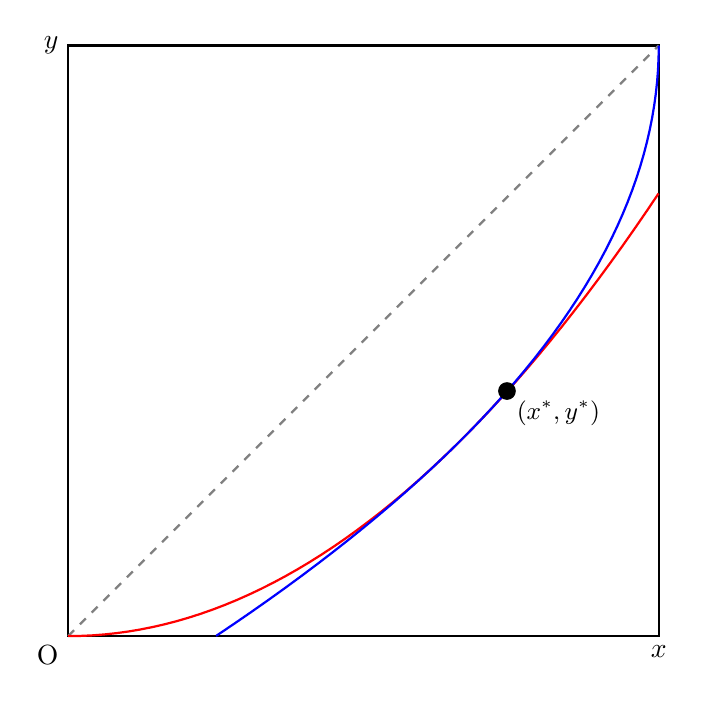
\begin{tikzpicture}[scale=7.5]
    % Square box [0,1] x [0,1]
    \draw[thick] (0, 0) rectangle (1, 1);
    
    % Axis labels
    \node[below left] at (0, 0) {O};
    \node[below] at (1, 0) {$x$};
    \node[left] at (0, 1) {$y$};
    
    % Diagonal y=x dashed line
    \draw[dashed, gray, thick] (0, 0) -- (1, 1);
    
    % Red curve: y = 3/4 * x^2 from (0,0) to (1, 3/4)
    \draw[red, thick] plot[domain=0:1, samples=50] (\x, {0.75*\x*\x});
    
    % Blue curve: symmetric to red curve about y=1-x
    % Parametric form: (1-0.75*t^2, 1-t) for t from 0 to 1
    \draw[blue, thick] plot[parametric, domain=0:1, samples=50] ({1-0.75*\x*\x}, {1-\x});
    
    % Intersection point (x*, y*)
    \def\xstar{0.743}
    \def\ystar{0.415}
    \fill[black] (\xstar, \ystar) circle (0.015);
    % \draw[dashed] (\xstar, \ystar) -- (\xstar, 0);
    % \draw[dashed] (0, \ystar) -- (\xstar, \ystar);
    \node[below right, font=\small] at (\xstar, \ystar) {$(x^*, y^*)$};
  \end{tikzpicture}
  \end{center}

  Let $(x^*,y^*)$ be the solution to
  \[
  \begin{aligned}
    u_1(y) & = \delta u_1(x)\\
    u_2(1-x) & = \delta u_2(1-y)
  \end{aligned}
  \]
  Player 1 always offers $x^*$, and rejects Player 2's offer if $y<x^*$. Player 2 always offers $y^*$, and rejects Player 1's offer if $x>y^*$. 

  $(z,t)$ is an outcome if a split of $(z,1-z)$ is accepted in period $t$.

  Define $v_1(z,t)$ as the dollar amount such that Player 1 is indifferent between receiving $v_1(z,t)$ today and receiving $z$ in period $t$. 
  \[
  u_1(v_1(z,t)) = \delta^{t-1} u_1(z).
  \]
  
  Define $v_2(z,t)$ as the dollar amount such that Player 2 is indifferent between giving Player 1 $v_2(z,t)$ today and giving Player 1 $z$ in period $t$. 
  \[
  u_2(1-v_2(z,t)) = \delta^{t-1} u_2(1-z).
  \]

  Define 
  \[
  \begin{aligned}
    M_i & = \sup\brace{v_i(z,t): (z,t) \text{ is a SPE of }G_i},\\
    m_i & = \inf\brace{v_i(z,t): (z,t) \text{ is a SPE of }G_i},
  \end{aligned}
  \]
  where $G_i$ is the subgame starting with Player $i$'s proposal.

  \clmp{}{
    \[
    u_1(M_2)\le \delta u_1(M_1).
    \]
  }{
    If Player 2 offers $y$ such that $u_1(y) > \delta u_1(M_1)$, then Player 1 would accept the offer, because the right hand side $\delta u_1(M_1)$ is the most that Player 1 can get in the subsequent $G_1$. So Player 2 would never offer such $y$. Hence, we must have $u_1(M_2)\le \delta u_1(M_1)$.
  }
  \clmp{}{
    \[
    u_1(M_2)\ge \delta u_1(M_1).
    \]
  }{
    If Player 2 offers $y$ such that $u_1(y) < \delta u_1(M_1)$, then Player 1 will reject the offer, because by rejecting and entering $G_1$, Player 1 can get at most $M_1$ (with current payoff equivalent $\delta u_1(M_1)$). Therefore, any successful offer in $G_2$ must satisfy $u_1(y) \ge \delta u_1(M_1)$. Taking the supremum over all $y$ in $G_2$ equilibria, we have $u_1(M_2)\ge \delta u_1(M_1)$.
  }
  \clmp{}{
    \[
    u_2(1-M_1)\ge \delta u_2(1-M_2).
    \]
  }{
    In $G_1$, if Player 1 demands more than $v_2(M_2,2)$, then Player 2 will reject. This implies
    \[
    M_1\le v_2(M_2,2).
    \]
    And this implies
    \[
    u_2(1-M_1)\ge u_2(1-v_2(M_2,2)) = \delta u_2(1-M_2).
    \]
  }
}

\section{Unequal Discounting}

Suppose now Player 1 has utility function $w_1$ and discount factor $\delta_1$, and Player 2 has utility function $w_2$ and discount factor $\delta_2$, with $\delta_1 < \delta_2$. We make the following transformation of the original problem:
\begin{itemize}
  \item Player 2 has $u_2 = w_2$ and $\delta = \delta_2$.
  \item Player 1 has $u_1 = \br{w_1(x)}^{\frac{\ln \delta_2}{\ln \delta_1}}$ and $\delta  = \delta_2$. (Note that $\frac{\ln \delta_2}{\ln \delta_1} < 1$ so that $u_1$ is concave, and is even ``more concave'' than $w_1$.)
\end{itemize}

Without loss of generality, assume that
\[
\begin{aligned}
  & \delta_1^{t-1}w_1(z)>\delta_1^{t'-1}w_1(z')\\
  \iff & \br{\delta_1^{t-1}w_1(z)}^{\frac{\ln \delta_2}{\ln \delta_1}}>\br{\delta_1^{t'-1}w_1(z')}^{\frac{\ln \delta_2}{\ln \delta_1}}\\
  \iff & \frac{\ln \delta_2}{\ln \delta_1}\br{(t-1)\ln \delta_1+ \ln w_1(z)} > \frac{\ln \delta_2}{\ln \delta_1} \br{(t'-1)\ln \delta_1+ \ln w_1(z')}\\
  \iff & (t-1)\ln \delta_2 + \frac{\ln \delta_2}{\ln \delta_1}\ln w_1(z) > (t'-1)\ln \delta_2 + \frac{\ln \delta_2}{\ln \delta_1}\ln w_1(z')\\
  \iff & \ln \delta_2^{t-1} + \ln \br{w_1(z)}^{\frac{\ln \delta_2}{\ln \delta_1}} > \ln \delta_2^{t'-1} + \ln \br{w_1(z')}^{\frac{\ln \delta_2}{\ln \delta_1}}\\
  \iff & \delta_2^{t-1}u_1(z) > \delta_2^{t'-1}u_1(z').
\end{aligned}
\]

